% ファイル名は「番号_タイトル.tex」
% 番号はNotionを参考
\newpage
\section{座談会}  % 割り振りの名前を記入

\subsection{場所・人員配置}
\begin{table}[h]
  \centering
  \begin{minipage}[t]{0.48\columnwidth}
    \centering
    \caption{場所・該当グループ}
    % グループは2/10に分けたやつです．企画書班のNotionにも追加しておくので参考にしておいてください．
    \begin{tabular}{cl}
      \hline
      場所 & K101 \\
      \hline
      グループ & 全員 \\
      \hline
    \end{tabular}
  \end{minipage}
  \begin{minipage}[t]{0.48\columnwidth}
    \centering
    \caption{役割分担}
    \begin{tabular}{ll}
      \hline
      \multicolumn{1}{c}{役割} & \multicolumn{1}{c}{担当者} \\
      \hline
      司会 & 細川夏風 \\
      話す人 & 全員 \\
      \hline
    \end{tabular}
  \end{minipage}
\end{table}

\subsection{詳細タイムスケジュール}
\vspace{0.5em}
\fontsize{8pt}{12pt}\selectfont

\begin{longtable}[c]{|p{.04\textwidth}|p{.2\textwidth}|p{.25\textwidth}|p{.45\textwidth}|}
  \caption{スケジュール} \\
  \hline
  \multicolumn{1}{|c|}{時間} & \multicolumn{1}{c|}{担当} & \multicolumn{1}{c|}{内容} & \multicolumn{1}{c|}{備考} \\
  \hline
  \endfirsthead
  
  \hline
  \multicolumn{1}{|c|}{時間} & \multicolumn{1}{c|}{担当} & \multicolumn{1}{c|}{内容} & \multicolumn{1}{c|}{備考} \\
  \hline
  \endhead
  
  \hline
  \endfoot
  
  \hline
  \endlastfoot

  \begin{tpacol}
    14:30
  \end{tpacol}&
  \begin{tpbcol}
    司会
  \end{tpbcol}&
  \begin{tpccol}
    座談会開始のお知らせ
  \end{tpccol}&
  \begin{tpdcol}
  \end{tpdcol}\\
  
  \begin{tpacol}

  \end{tpacol}&
  \begin{tpbcol}
    それぞれの話題話す人たち
  \end{tpbcol}&
  \begin{tpccol}
    各場所に移動する
  \end{tpccol}&
  \begin{tpdcol}
    
  \end{tpdcol}\\

\end{longtable}
\normalsize

\begin{figure}[h]
  \centering
  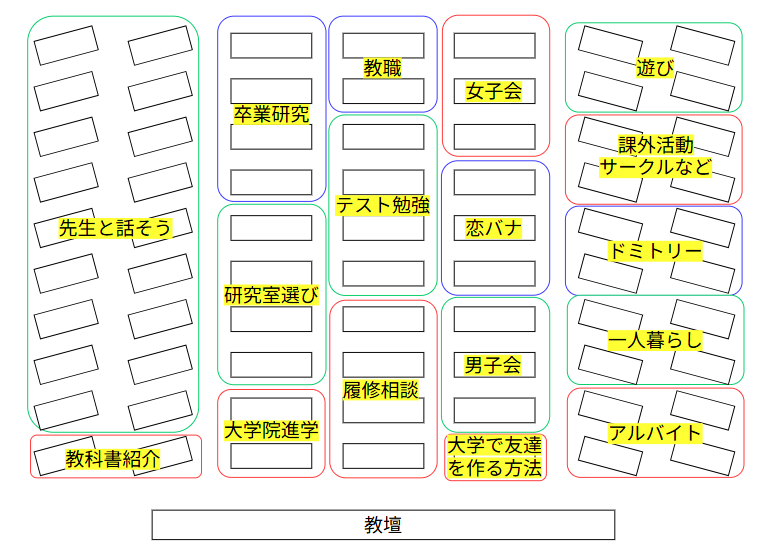
\includegraphics[width=0.8\textwidth]{document/3_Deta/zadankai_zaseki.png}
  \caption{座談会のイメージ図}
\end{figure}

\subsection{準備物品}
\begin{table}[h]
  \centering
  \caption{物品}
  \begin{tabular}{lrl}
    \hline
    \multicolumn{1}{c}{物品} & \multicolumn{1}{c}{数量} & \multicolumn{1}{c}{使用用途・備考} \\
    \hline
    
    \hline
  \end{tabular}
\end{table}

\subsection{備考}
情報学群の公式行事であるので適当なことは言わない．

責任に関しては情報学群が責任を負うことは忘れないように．

マウントとか自慢とかはしないように
% 特に書くことなければ省略してOK